\documentclass[a4paper,12pt]{article}

\usepackage{graphicx}

\begin{document}

\title{Service Oriented Architecture Proposal}
\author{
  De Smet, Rafael \\
  \texttt{rafael.desmet@student.uantwerpen.be}
  \and
  Keerthana Sanala Prakash \\
  \texttt{keerthana.sanalaprakash@student.uantwerpen.be}
  \and
  Jordan Parezys \\
  \texttt{jordan.parezys@student.uantwerpen.be}
}
\date{}
\maketitle

\section{Introduction}

In this document we propose our architecture design for the social network application we have to build for Distributed Computing. It shows which microservices we plan to use and how they are connected to each other.

\section{High-Level Service Composition Diagram}

Below is the high-level diagram, showing the microservices and the links between them.

\section{Detailed Service Profile}

\subsection{Front App}

This service will handle the presentation side of the full application. Here we will develop the news feed, the user profiles, showing of the advertisements. The messaging service will be accessible in the full application. This front end service will use all the back end services to show the right content to the user. We will mainly focus on the web application and not on the mobile application (included in the diagram to be complete, but not really a goal).
\newline
\newline
We suggest to use Angular to create the front end.

\subsection{Standalone Messaging Service}

We will also provide a standalone messaging service that can be used independently from the full application. This front end service will have access to the back-end messaging, notification and user services. It has no need to have access to the content analysing service for instance.
\newline
\newline
We suggest to use Angular to create the front end.

\subsection{Login And Registration Service}

This service will manage the registration of new users and the login of existing users. It will have access to a database that holds all the users registered on the application.
\newline
\newline
This service is linked with the User Service and the Admin Service.
\newline
\newline
For the database we suggest to use SQLAlchemy in Python. For the microservice itself Flask and Python seems suitable.

\subsection{Photo Service}

This service will handle everything a user can do with a photo. A photo can be posted, liked, people can be tagged in one or deleted. A separate database is provided for the photos.
\newline
\newline
This service is linked with the User Service, the Post Service and the Admin Service.
\newline
\newline
For the database we suggest to use SQLAlchemy in Python. For the microservice itself Flask and Python seems suitable.

\subsection{User Service}

This service will handle everything concerning the information of a user. This will control what the user shows on his profile, his information, posts, comments and photos. This service is the most linked of all because it groups lot of information from several other services. It is linked with the Login Service (can only have a profile if it is a registered user), with the Photo Service, the Post Service, the Comment Service, the Advertisement Service (to see personalized ads), the Messaging Service and the Admin Service. Relationships between users, like friends and people to follow or people who you don't want to see are handled here and stored in a dedicated database. Other data is requested from the other services' databases.
\newline
\newline
A distinction between administrators and regular users is made.

\subsection{Messaging Service}

This service handles the messaging between two users. This will be used as a standalone application and as a part of the full application in the front end. In the back end this will have no difference. The service will allow for two users to privately message. For this we need a database that holds every conversation between every pair of users. When a new message is sent by one of the users in the conversation, the other will receive a notification.
\newline
\newline
This service is linked with the User Service, the Notification Service and the Admin Service

\subsection{Post Service}

A user can post some text to the application. It will be shown on the user's profile and on the news feed. This will be handled here with a dedicated database for the text posts a user makes. If the user wants to post a photo it will use the Photo Service. When a user posts something, other users who follow this user can get a notification. Other users can leave comments on a post.\newline
\newline
This service is linked with the User Service, the Photo Service, the Notification Service, the News Feed Service, the Comment Service and the Admin Service.

\subsection{Advertisement Service}

This service will analyse a user's profile, posts and comments and show a personalized advertisement for this user only, on its news feed. All the possible advertisements to show are stored in a dedicated database.
\newline
\newline
Therefore this service is linked with the User Service, the News Feed Service, the Recommendation Service and the Admin Service.

\subsection{Content Analysing Service}

Every post a user makes is being analysed for cyber bullying. If there is a bad word or phrase detected, the user will get a notification that asks whether or not they really want to post this. The dictionaries used to do the analysing of a post are stored in a dedicated database.
\newline
\newline
Therefore it is linked with the Notification Service, the Post service and the Admin Service.

\subsection{Recommendation Service}

This service keeps information on the user's preferences so it can determine what ads the advertisement service can use. These preferences are stored in a separate database. Therefore this is linked to the Advertisement Service and to the Admin Service.

\subsection{Notification Service}

The Notification Service trigger the notifications for a user. This can be either that a user has messaged you, or that someone has posted, that someone commented on a post, or your post was analysed and a bad word found, etc. We keep track of the notifications made for a user in a separate database.
\newline
\newline
This is linked to the User Service, the Post Service, the Content Analysing Service, the Messaging Service, the Comment Service and the Admin Service.

\subsection{News Feed Service}

The news feed will show the posts and photos of other users, together with the comments and people tagged (in photos) of each post. The advertisements are shown here as well. We don't need a dedicated database because we get all the data from other services. This service is linked with the Post Service, the Advertisement Service, the Comment Service, the Photo Service and the Admin Service.

\subsection{Comment Service}

The comment service will hold all the comments users make on posts and photos. When a new comment is made on a post or photo, a notification is sent to the correct user and shown in the news feed. So we need a dedicated database and links to the Photo Service, the Post Service, the User Service, the News Feed Service, the Notification Service and the Admin Service. 

\subsection{Administration Management Service}

This is a special service because it is only accessible for the administrators of the application. An admin can access any service (and therefore this service is linked with all the other ones) and perform the corresponding actions (delete user, comments, posts, photos; add new advertisements; make posts, etc). There is no need for a separate database because we use the data from the other services.

\newpage

\begin{figure}
  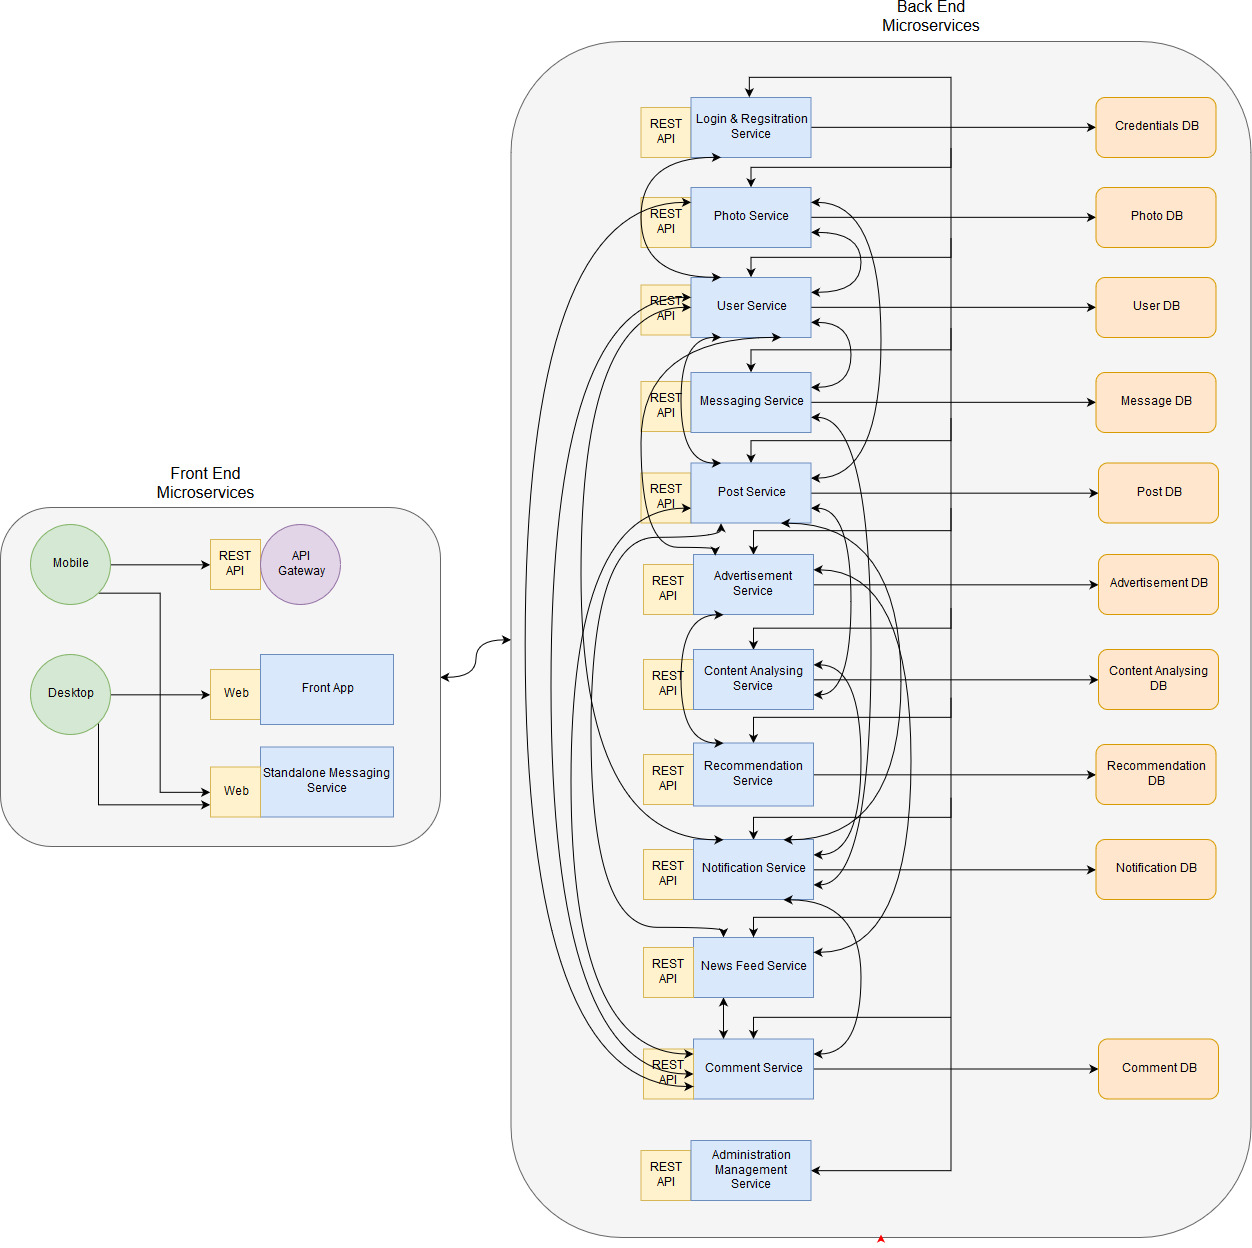
\includegraphics[width=\linewidth]{architectureSchema.jpg}
\end{figure}

\end{document}